\section{Tutorial B5B}

\begin{problem}
    The equation of a closed curve is $(x+2y)^2 + 3(x-y)^2 = 27$.

    \begin{enumerate}
        \item Show, by differentiation, that the gradient at the point $(x,y)$ on the curve may be expressed in the form $\der{y}{x} = \frac{y-4x}{7y-x}$.
        \item Find the equations of the tangents to the curve that are parallel to
        \begin{enumerate}
            \item the $x$-axis,
            \item the $y$-axis.
        \end{enumerate}
    \end{enumerate}
\end{problem}
\begin{solution}
    \begin{ppart}
        Implicitly differentiating the given equation, \[(x+2y)\bp{1 + 2y'} + 3(x-y)(1 - y') = (-x + 7y)y' + 4x - y = 0 \implies y' = \frac{y-4x}{7y-x}.\]
    \end{ppart}
    \begin{ppart}
        \begin{psubpart}
            When the tangent to the curve is parallel to the $x$-axis, $y' = 0$, whence $y = 4x$. Substituting $y=4x$ into the given equation, \[(9x)^2 + 3(-3x)^2 = 27 \implies 108x^2 = 27 \implies x^2 = \frac14 \implies x = \pm \frac12 \implies y = \pm 2.\] The equations of the tangents are hence $y = \pm 2$.
        \end{psubpart}
        \begin{psubpart}
            When the tangent to the curve is parallel to the $y$-axis, $y'$ is undefined. Hence, $7y-x =0 \implies x = 7y$. Substituting $x = 7y$ into the given equation, \[(9y)^2 + 3(6y)^2 = 27 \implies 189y^2 = 27 \implies y^2 = \frac17 \implies y = \pm \frac1{\sqrt7} \implies x = \pm \sqrt7.\] The equations of the tangents are hence $x = \pm \sqrt7$.
        \end{psubpart}
    \end{ppart}
\end{solution}

\begin{problem}
    A piece of wire of length 8 cm is cut into two pieces, one of length $x$ cm, the other of length $(8-x)$ cm. The piece of length $x$ cm is bent to form a circle with circumference $x$ cm. The other piece is bent to form a square with perimeter $(8-x)$ cm. Show that, as $x$ varies, the sum of the areas enclosed by these two pieces of wire is a minimum when the radius of the circle is $\frac4{4+\pi}$ cm.
\end{problem}
\begin{solution}
    Let the radius of the circle be $r$ cm. Then we have $x = 2\pi r \implies r = x/2\pi$. Let the side length of the square be $s$ cm. Then we have $8-x=4s \implies s = 2-x/4$. Let the total area enclosed by the circle and the square be $A(x)$. \[A(x) = \pi r^2 + s^2 = \pi \bp{\frac{x}{2\pi}}^2 + \bp{2-\frac{x}4}^2 = \bp{\frac1{4\pi} + \frac1{16}}x^2 - x + 4.\] Consider the stationary points of $A(x)$. For stationary points, $A'(x) = 0$. \[A'(x) = \bp{\frac1{2\pi} + \frac1{8}}x - 1 = 0 \implies x = \frac1{\frac1{2\pi} + \frac1{8}} = \frac{8\pi}{4 + \pi}.\]

    \begin{table}[H]
        \centering
        \begin{tabular}{|c|c|c|c|}
        \hline
        $x$ & $\bp{\frac{8\pi}{4 + \pi}}^-$ & $\frac{8\pi}{4 + \pi}$ & $\bp{\frac{8\pi}{4 + \pi}}^+$ \\\hline
        $\derx{A}{x}$ & $-$ve   & 0 & +ve   \\\hline
        \end{tabular}
    \end{table}

    Hence, by the first derivative test, the minimum value of $A(x)$ is achieved when $x = \frac{8\pi}{4 + \pi}$, whence \[r = \frac{1}{2\pi} \cdot \frac{8\pi}{4 + \pi} = \frac{4}{4+\pi} \text{ cm}.\]
\end{solution}

\begin{problem}
    A spherical balloon is being inflated in such a way that its volume is increasing at a constant rate of 150 cm$^3$s$^{-1}$. At time $t$ seconds, the radius of the balloon is $r$ cm.

    \begin{enumerate}
        \item Find $\derx{r}{t}$ when $r = 50$.
        \item Find the rate of increase of the surface area of the balloon when its radius is 50 cm.
    \end{enumerate}
\end{problem}
\begin{solution}
    Let the volume of the balloon be $V(r) = \frac43 \pi r^3$ cm$^3$.

    \begin{ppart}
        Note that $\der{V}{t} = 150$ and $\der{V}{r} = 4\pi r^2$. \[\der{r}{t} = \frac{\derx{r}{V}}{\derx{t}{V}} = \frac{\derx{V}{t}}{\derx{V}{r}} = \frac{150}{4\pi r^2} = \frac{75}{2\pi r^2}.\] Evaluating $\der{r}{t}$ at $r=50$, \[\evalder{\der{r}{t}}{r=50} = \frac{75}{2 \pi \cdot 50^2} = \frac3{200\pi}.\]
    \end{ppart}
    \begin{ppart}
        Let the surface area of the balloon be $A(r) = 4\pi r^2$. Observe that $\der{A}{r} = 8 \pi r$. \[\der{A}{t} = \der{A}{r} \cdot \der{r}{t} \implies \evalder{\der{A}{t}}{r=50} = \bp{8\pi\cdot50}\bp{\frac3{200\pi}} = 6.\] Thus, the rate of increase of the surface area of the balloon when its radius is 50 cm is 6 cm/s.
    \end{ppart}
\end{solution}

\begin{problem}
    A curve has parametric equations $x = 5\sec\t, \, y = 3\tan\t$, where $-\frac12\pi < \t < \frac12\pi$. Find the exact coordinates of the point on the curve at which the normal is parallel to the line $y=x$.
\end{problem}
\begin{solution}
    Observe that $x^2 = 25\sec^2\t$ and $\frac{25}9 y^2 = 25\tan^2\t$. Using the identity $\tan^2\t + 1 = \sec^2\t$, we get \[\frac{25}9 y^2 + 25 = x^2. \tag{$\ast$}\] Implicitly differentiating with respect to $x$, we get \[\frac{25}9 y \cdot y' = x.\] Since the normal is parallel to $y =x$, the tangent is parallel to $y = -x$, whence $y' = -1$. Thus, \[y = -\frac9{25} x.\] Substituting $y = -\frac9{25}x$ into ($\ast$), \[\frac{25}9 \bp{-\frac9{25} x}^2 + 25 = x^2 \implies \frac{16}{25} x^2 = 25 \implies \frac45 x = \pm 5 \implies x = \pm \frac{25}4.\] Observe that for $-\pi/2 < \t < \pi/2$, $x=5\sec\t \geq 5$. We thus take $x=25/4$, whence $y = -9/4$. The coordinate of the required point is thus $\bp{25/4, -9/4}$.
\end{solution}

\begin{problem}
    The parametric equations of a curve are \[x = t^2, \, y = \frac2t.\]
    \begin{enumerate}
        \item Find the equation of the tangent to the curve at the point $(p^2, 2/p)$, simplifying your answer.
        \item Hence, find the coordinates of the points $Q$ and $R$ where this tangent meets the $x$- and $y$-axes respectively.
        \item The point $F$ is the mid-point of $QR$. Find a Cartesian equation of the curve traced by $F$ as $p$ varies.
    \end{enumerate}
\end{problem}
\begin{solution}
    \begin{ppart}
        Observe that $\derx{x}{t} = 2t$ and $\derx{y}{t} = -2/t^2$. Hence, \[\der{y}{x} = \frac{\derx{y}{t}}{\derx{x}{t}} = \frac{-2/t^2}{2t} = -\frac1{t^3}.\] Using the point-slope formula, the tangent to the curve at $(p^2, 2/p)$ is given by the equation \[y - \frac2p = -\frac1{p^3} \bp{x - p^2} \implies y = \frac3p - \frac1{p^3} x.\]
    \end{ppart}
    \begin{ppart}
        Consider the case where $y = 0$: \[0 = \frac3p - \frac1{p^3} x \implies x = 3p^2 \implies Q\bp{3p^2, 0}.\]

        Consider the case where $x = 0$: \[y = \frac3p \implies R\bp{0, \frac3p}.\]
    \end{ppart}
    \begin{ppart}
        Note that \[F = \bp{\frac32 p^2, \frac3{2p}}.\] As $p$ varies, $F$ traces a curve given by the parametric equations $x = 3p^2/2$, $y = 3/2p$. Hence, \[p^2 = \frac23 x = \frac{9}{4y^2} \implies y^2 = \frac{27}{8x}.\]
    \end{ppart}
\end{solution}

\begin{problem}
    \begin{center}\tikzsetnextfilename{289}
        \begin{tikzpicture}
            \draw (0,0) arc[x radius=2, y radius=2, start angle=180, end angle=0];

            \draw (0, 0) -- (0, -2);

            \draw (4, 0) -- (4, -2);

            \draw (0, -2) -- (4, -2);

            \draw[dotted, thick] (0, 0) -- (4, 0);

            \node[anchor=east] at (0, -1) {$y$};

            \node[anchor=north] at (2, -2) {$x$};
        \end{tikzpicture}    
    \end{center}
    
    A new flower-bed is being designed for a large garden. The flower-bed will occupy a rectangle $x$ m by $y$ m together with a semicircle of diameter $x$ m, as shown in the diagram. A low wall will be built around the flowerbed. The time needed to build the wall will be 3 hours per metre for the straight parts and 9 hours per metre for the semicircular part. Given that a total time of 180 hours is taken to build the wall, find, using differentiation, the values of $x$ and $y$ which give a flower-bed of maximum area.
\end{problem}
\begin{solution}
    Observe that the length of the straight parts is $(2y + x)$ m, while the length of the semicircular part is $\frac12 \pi x$ m. Since a total time of 180 hours is taken to build the wall, \[3 (2y + x) + 9\bp{\frac12 \pi x} = 180 \implies 4y + 2x + 3 \pi x = 120 \implies x = \frac{120-4y}{2+3\pi}.\] Differentiating with respect to $y$, we get $x' = -4/(2 + 3\pi)$. Let $A(y)$ be the total area enclosed by the garden, in m$^2$. Observe that \[A(y) = xy + \frac12 \pi \bp{\frac{x}2}^2 = xy + \frac\pi8 x^2.\] Consider the stationary points of $A(y)$. For stationary points, $A'(y) = 0$. \[A'(y) = \bp{x' y + x} + \frac\pi4 x \cdot x' = 0.\] Substituting in our values of $x$ and $x'$, we get \[\bs{y\bp{-\frac{4}{2 + 3\pi}} + \frac{120-4y}{2+3\pi}} + \bs{\frac\pi4 \bp{\frac{120-4y}{2+3\pi}} \bp{-\frac{4}{2 + 3\pi}}} = 0.\] Using G.C., we get $y = 12.6 \tosf{3}$, whence $x = 6.09 \tosf{3}$.
\end{solution}

\begin{problem}
    \begin{center}\tikzsetnextfilename{290}
        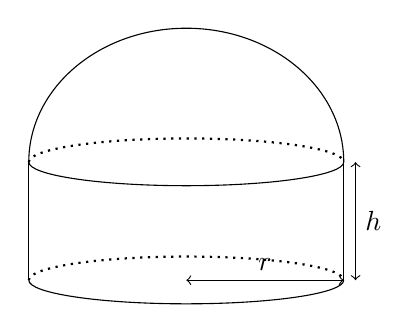
\begin{tikzpicture}
            \draw (0,0) arc[x radius=2, y radius=1.7, start angle=180, end angle=0];

            \draw (0, 0) arc[x radius=2, y radius=0.3, start angle=-180, end angle=0];

            \draw[dotted, thick] (0, 0) arc[x radius=2, y radius=0.3, start angle=180, end angle=0];

            \draw (0, 0) -- (0, -1.5);

            \draw (4, 0) -- (4, -1.5);

            \draw (0, -1.5) arc[x radius=2, y radius=0.3, start angle=-180, end angle=0];

            \draw[dotted, thick] (0, -1.5) arc[x radius=2, y radius=0.3, start angle=180, end angle=0];

            \draw[<->] (2, -1.5) -- (4, -1.5);

            \node[anchor=south] at (3, -1.5) {$r$};

            \draw[<->] (4.15, 0) -- (4.15, -1.5);

            \node[anchor=west] at (4.15, -0.75) {$h$};
        \end{tikzpicture}    
    \end{center}

    A model of a concert hall is made up of three parts.

    \begin{itemize}
        \item The roof is modelled by the curved surface of a hemisphere of radius $r$ cm.
        \item The walls are modelled by the curved surface of a cylinder of radius $r$ cm and height $h$ cm.
        \item The floor is modelled by a circular disc of radius $r$ cm.
    \end{itemize}

    The three parts are joined together as shown in the diagram. The model is made of material of negligible thickness.

    \begin{enumerate}
        \item It is given that the volume of the model is a fixed value $k$ cm$^3$, and the external surface area is a minimum. Use differentiation to find the values of $r$ and $h$ in terms of $k$. Simplify your answers.
        \item It is given instead that the volume of the model is 200 cm$^3$ and its external surface area is 180 cm$^2$. Show that there are two possible values of $r$. Given also that $r < h$, find the value of $r$ and the value of $h$.
    \end{enumerate}
\end{problem}
\begin{solution}
    \begin{ppart}
        Let the volume of the model be $V$ cm$^3$. Then \[V = \frac12\bp{\frac43 \pi r^3} + \pi r^2 h = k \implies h = \frac{k}{\pi r^2}-\frac23 r. \tag{1}\] Let the external surface area of the model be $A$ cm$^2$. Then \[A = \frac{4\pi r^2}2 + 2\pi r h + \pi r^2 = 3\pi r^2 + 2\pi r\bp{\frac{k}{\pi r^2}-\frac23 r} = \frac{5\pi}3 r^2 + \frac{2k}{r}. \tag{2}\] Consider the stationary points of $A$. For stationary points, $\derx{A}{r} = 0$. \[\der{A}{r} = \frac{10\pi}3 r - \frac{2k}{r^2} = 0 \implies r^3 = \frac{3k}{5\pi} \implies r = \sqrt[3]{\frac{3k}{5\pi}}.\]

        \begin{table}[H]
            \centering
            \begin{tabular}{|c|c|c|c|}
            \hline
            $r$ & $\sqrt[3]{\frac{3k}{5\pi}}^-$ & $\sqrt[3]{\frac{3k}{5\pi}}$ & $\sqrt[3]{\frac{3k}{5\pi}}^+$ \\\hline
            $\derx{A}{r}$ & $-$ve   & 0 & +ve   \\\hline
            \end{tabular}
        \end{table}
        Hence, by the first derivative test, $A$ is at a minimum when $r = \sqrt[3]{\frac{3k}{5\pi}}$.

        Substituting $r^3 = \frac{3k}{5\pi}$ into (1), \[\frac23 \pi \bp{\frac{3k}{5\pi}} + \pi r^2 h = \frac{2}{5}k + \pi r^2h = k \implies r^2 h = \frac{3k}{5\pi} = r^3 \implies h = r = \sqrt[3]{\frac{3k}{5\pi}}.\]
    \end{ppart}
    \begin{ppart}
        From (2), we have \[\frac{5\pi}3 r^2 + \frac{2(200)}{r} = 180 \implies \pi r^3 - 108r + 240 = 0.\] Let $f(r) = \pi r^3 - 108r + 240$. Consider the stationary points of $f(r)$. For stationary points, $f'(r) = 0$. \[f'(r) = 3\pi r^2 - 108 = 0 \implies r^2 = \frac{36}{\pi} \implies r = \pm \frac6{\sqrt\pi}.\] Since $f(r)$ is a cubic with two turning points, it follows that there is exactly one root in each of the following three intervals: \[\bp{-\infty, -\frac6{\sqrt\pi}}, \quad \bp{-\frac6{\sqrt\pi}, \frac6{\sqrt\pi}}, \quad \bp{\frac6{\sqrt\pi}, \infty}.\] We now show that the root in the interval $\bp{-\frac6{\sqrt\pi}, \frac6{\sqrt\pi}}$ is positive. Since $f(r)$ has a positive leading coefficient, it must be decreasing in the interval $\bp{-\frac6{\sqrt\pi}, \frac6{\sqrt\pi}}$. Since $f(0) = 240 > 0$, the root in said interval must be positive. Hence, $f(r) = 0$ has two positive roots. Using G.C., the roots are $r = 3.04$ and $r = 3.72$. From (1), we know that \[h = \frac{200}{\pi r^2} - \frac23 r.\] When $r = 3.04$, $h = 4.88 > r$. When $r = 3.72$, $h = 2.12 < r$. Thus, given that $r < h$, we have $r = 3.04$ and $h = 4.88$.
    \end{ppart}
\end{solution}

\clearpage
\begin{problem}
    \begin{center}\tikzsetnextfilename{291}
        \begin{tikzpicture}
            \draw[dotted, thick] (0, 0) -- (3, 0);

            \draw (3, 0) -- (3, 2);

            \draw[very thick] (3, 2) -- (3, 5);

            \draw (0, 0) -- (3, 5);

            \draw (0, 0) -- (3, 2);

            \draw (0, 0) -- (0, -0.5);

            \draw (0, -0.5) -- (3, -0.5);

            \draw (3, -0.5) -- (3, 0);

            \draw[<->] (3.15, -0.5) -- (3.15, 2);

            \node[anchor=west] at (3.15, 0.75) {4 m};

            \draw[<->] (3.15, 2) -- (3.15, 5);

            \node[anchor=west] at (3.15, 3.5) {6 m};

            \draw[<->] (-0.15, 0) -- (-0.15, -0.5);

            \node[anchor=east] at (-0.15, -0.25) {1 m};

            \draw (0.5, 0) arc[x radius=0.5, y radius=0.5, start angle=0, end angle=59];

            \node at (0.65, 0.2) {$y$};

            \node at (0.5, 0.53) {$\t$};
        \end{tikzpicture}
    \end{center}
    
    A movie screen on a vertical wall is 6 m high and 4 m above the horizontal floor. A boy who is standing at $x$ m away from the wall has eye level at 1 m above the floor as shown in the diagram.

    The viewing angle of the boy at that position is $\t$ and the angle of elevation of the bottom of the screen is $y$.

    \begin{enumerate}
        \item Express $y$ in terms of $x$.
        \item By expressing $\t$ in terms of $x$ or otherwise, find the stationary value of $\t$, giving your answers in exact form. Determine if the value is a maximum or minimum value, showing your working clearly.
    \end{enumerate}
\end{problem}
\begin{solution}
    \begin{ppart}
        Observe that $\tan y = 3/x$, whence $y = \arctan{3/x}$.
    \end{ppart}
    \begin{ppart}
        Observe that $\tan(y + \t) = 9/x$. Hence, \[\tan{y + \t} = \frac{\tan y + \tan \t}{1 - \tan y \tan \t} = \frac{3/x + \tan \t}{1 - (3/x) \tan \t} = \frac{3 + x\tan\t}{x - 3\tan\t} = \frac9x \implies \tan \t = \frac{6x}{x^2 + 27}.\] Hence, \[\t = \arctan{\frac{6x}{x^2 + 27}}.\] Differentiating with respect to $x$, \[\der{\t}{x} = \frac{1}{1 + \bp{\frac{6x}{x^2 + 27}}^2} \bs{\frac{6\bp{x^2 + 27} - 6x(2x)}{\bp{x^2 + 27}^2}} = \frac{-6x^2 + 162}{36x^2 + \bp{x^2+27}^2}.\] For stationary points, $\derx{\t}{x} = 0$. Hence, \[-6x^2 + 162 = 0 \implies x^2 = 27 \implies x = \pm 3\sqrt3.\] Since $x > 0$, we only take $x = 3\sqrt{3}$. Thus, \[\t = \arctan{\frac{6\bp{3\sqrt3}}{27 + 27}} = \arctan{\frac1{\sqrt3}} = \frac\pi6.\]
        \begin{table}[H]
            \centering
            \begin{tabular}{|c|c|c|c|}
            \hline
            $x$ & $3\sqrt{3}^-$ & $3\sqrt{3}$ & $3\sqrt{3}^+$ \\\hline
            $\derx{\t}{x}$ & +ve   & 0 & $-$ve   \\\hline
            \end{tabular}
        \end{table}
        Thus, by the first derivative test, $\t = \frac{\pi}6$ is a maximum value.
    \end{ppart}
\end{solution}

\begin{problem}
    \begin{center}\tikzsetnextfilename{292}
        \begin{tikzpicture}
            \draw (0, 0) circle[radius=sqrt(3)];

            \draw (-1.5, 0.5*sqrt 3) arc[x radius=1.5, y radius=0.3, start angle=-180, end angle=0];

            \draw[dotted, thick] (-1.5, 0.5*sqrt 3) arc[x radius=1.5, y radius=0.3, start angle=180, end angle=0];

            \draw (-1.5, 0.5*sqrt 3) -- (0, -sqrt 3);

            \draw (1.5, 0.5*sqrt 3) -- (0, -sqrt 3);

            \draw[dotted, thick] (0, 0.5*sqrt 3) -- (1.5, 0.5*sqrt 3);

            \node[anchor=south] at (0.75, 0.5*sqrt 3) {$r$};

            \draw[dotted, thick] (0, 0.5*sqrt 3) -- (0, -sqrt 3);

            \node[anchor=east] at (0, 0) {$h$};

            \draw (0, 0.5-sqrt 3) arc[x radius=0.5, y radius=0.5, start angle=90, end angle=60];

            \node at (0.20, 0.75-sqrt 3) {$\t$};
        \end{tikzpicture}    
    \end{center}

    The diagram shows a right inverted cone of radius $r$, height $h$ and semi-vertical angle $\t$, which is inscribed in a sphere of radius 1 unit.

    Prove that $r^2 = 2h - h^2$.

    \begin{enumerate}
        \item As $r$ and $h$ varies, determine the exact maximum volume of the cone.
        \item Show that $h = 2\cos^2\t$. The volume of the cone is increasing at a rate of 6 unit$^3$/s when $h = \frac32$. Determine the rate of change of $\t$ at this instant, leaving your answer in an exact form.
    \end{enumerate}
\end{problem}
\begin{solution}
    Consider the following diagram of the cone and sphere.

    \begin{center}\tikzsetnextfilename{293}
        \begin{tikzpicture}
            \draw (0, 0) circle[radius=sqrt(3)];

            \draw (-1.5, 0.5*sqrt 3) -- (1.5, 0.5*sqrt 3);

            \draw (-1.5, 0.5*sqrt 3) -- (0, -sqrt 3);

            \draw (1.5, 0.5*sqrt 3) -- (0, -sqrt 3);

            \draw[dotted, thick] (0, 0.5*sqrt 3) -- (1.5, 0.5*sqrt 3);

            \draw[<->] (0, 0.5 * sqrt 3 + 0.1) -- (1.5, 0.5*sqrt 3 + 0.1);

            \node[anchor=south] at (0.75, 0.5*sqrt 3) {$r$};

            \draw[dotted, thick] (0, 0.5*sqrt 3) -- (0, -sqrt 3);

            \node[anchor=east] at (0, 0) {$h$};

            \draw (0, 0.5-sqrt 3) arc[x radius=0.5, y radius=0.5, start angle=90, end angle=60];

            \node at (0.20, 0.75-sqrt 3) {$\t$};

            \node[anchor=north] at (0, -sqrt 3) {$O$};

            \node[anchor=west] at (1.5, 0.5 *sqrt 3) {$(r, h)$};

            \node[anchor=east, white] at (-1.5, 0.5 *sqrt 3) {$(r, h)$};
        \end{tikzpicture}    
    \end{center}

    Let the origin be the tip of the cone. Since the sphere has radius 1 unit, the circle is given by the equation $x^2 + (y-1)^2 = 1$. Since the point $(r, h)$ lies on the circle, \[r^2 + (h-1)^2 = 1 \implies r^2 = 2h - h^2\tag{$\ast$}.\]

    \begin{ppart}
        Implicitly differentiating ($\ast$) with respect to $r$, \[2r = 2\cdot\der{h}{r} - 2h \cdot \der{h}{r} \implies \der{h}{r} = \frac{r}{1-h}.\] Let the volume of the cone be $V(r)$ units$^3$. Then \[V(r) = \frac13 \pi r^2 h = \frac13 \pi \bp{2h - h^2} h = \frac13 \pi \bp{2h^2 - h^3}.\] Differentiating $V(r)$ with respect to $r$, \[V'(r) = \frac13 \pi \bp{4h \cdot \der{h}{r} - 3h^2 \cdot \der{h}{r}} = \frac13 \bp{\frac{\pi rh}{1-h}} (4 - 3h).\] Consider the stationary values of $V(r)$. For stationary values, $V'(r) = 0$, whence $h = 4/3$. Substituting this into ($\ast$), we obtain \[r^2 = 2\bp{\frac43} - \bp{\frac43}^2 = \frac89 \implies r = \sqrt{\frac89}.\] Note that we reject $r = -\sqrt{8/9}$ as $r > 0$.

        \begin{table}[H]
            \centering
            \begin{tabular}{|c|c|c|c|}
            \hline
            $r$ & $\sqrt{8/9}^-$ & $\sqrt{8/9}$ & $\sqrt{8/9}^+$ \\\hline
            $V'(r)$ & +ve   & 0 & $-$ve   \\\hline
            \end{tabular}
        \end{table}

        Hence, the maximum volume is achieved when $r = \sqrt{8/9}$. Note that \[V\bp{\sqrt{\frac89}} = \frac13 \pi \bp{\frac89}\bp{\frac43} = \frac{32}{81}\pi.\] The maximum volume of the cone is hence $32\pi/81$ units$^3$.
    \end{ppart}
    \begin{ppart}
        From the diagram, we have \[\cos\t = \frac{h}{\sqrt{r^2 + h^2}} \implies 2\cos^2 \t = \frac{2h^2}{r^2 + h^2} = \frac{2h^2}{2h - h^2 + h^2} = h.\]

        Observe that \[V = \frac\pi3 \bp{2h^2 - h^3} = \frac\pi3 \bp{8\cos^4 \t - 8\cos^6 \t} = \frac{8\pi}3 \bp{\cos^4 \t - \cos^6 \t}.\] Differentiating with respect to $\t$, we get \[\der{V}{\t} = \frac{8\pi}3 \bp{-4\cos^3 \t \sin \t + 6\cos^5 \t \sin \t} = \frac{16\pi}3 \cos^3 \t \sin \t \bp{-2 + 3 \cos^2 \t}.\] Since $2\cos^2 \t = h = 3/2$, we clearly have $\t = \pi/6$. Thus, \[\evalder{\der{V}{\t}}{h = 3/2} = \frac{16\pi}3 \cos^3 \frac\pi6 \sin \frac\pi6 \bp{-2 + 3\cos^2 \frac\pi6} = \frac{\sqrt 3 \pi}4.\] Hence, \[\evalder{\der{\t}{t}}{h = 3/2} = \evalder{\bp{\der{\t}{V} \cdot \der{V}{t}}}{h = 3/2} = \frac{6}{\sqrt3 \pi /4} = \frac{8\sqrt3}{\pi}.\] $\t$ is thus increasing at a rate of $8\sqrt3/\pi$ radians per second when $h = \frac32$.
    \end{ppart}
\end{solution}

\begin{problem}
    \begin{center}\tikzsetnextfilename{294}
        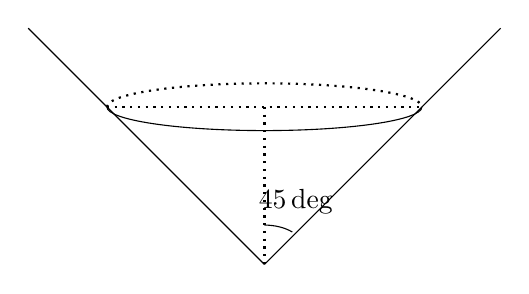
\begin{tikzpicture}
            \draw (0, 0) -- (-3, 3);

            \draw (0, 0) -- (3, 3);

            \draw(-2, 2) arc[x radius=2, y radius=0.3, start angle=-180, end angle=0];
            
            \draw[dotted, thick] (-2, 2) arc[x radius=2, y radius=0.3, start angle=180, end angle=0];

            \draw[dotted, thick] (-2, 2) -- (2, 2);

            \draw[dotted, thick] (0, 2) -- (0, 0);

            \draw (0, 0.5) arc[x radius=0.5, y radius=0.3, start angle=90, end angle=45];

            \node at (0.4, 0.8) {$45\deg$};
        \end{tikzpicture}    
    \end{center}

    A hollow cone of semi-vertical angle $45\deg$ is held with its axis vertical and vertex downwards. At the beginning of an experiment, it is filled with 390 cm$^3$ of liquid. The liquid runs out through a small hole at the vertex at a constant rate of 2 cm$^3$/s. 

    Find the rate at which the depth of the liquid is decreasing 3 minutes after the start of the experiment.
\end{problem}
\begin{solution}
    Consider the following diagram.

    \begin{center}\tikzsetnextfilename{295}
        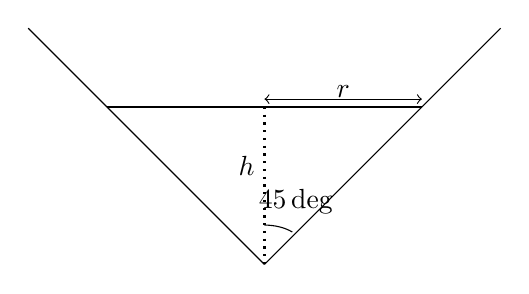
\begin{tikzpicture}
            \draw (0, 0) -- (-3, 3);

            \draw (0, 0) -- (3, 3);

            \draw (-2, 2) -- (2, 2);

            \draw[dotted, thick] (0, 2) -- (0, 0);

            \draw (0, 0.5) arc[x radius=0.5, y radius=0.3, start angle=90, end angle=45];

            \node at (0.4, 0.8) {$45\deg$};

            \node[anchor=east] at (0, 1.25) {$h$};

            \node[anchor=south] at (1, 2) {$r$};

            \draw[<->] (0, 2.1) -- (2, 2.1); 
        \end{tikzpicture}    
    \end{center}

    Let the volume of liquid be $V = \frac13 \pi r^2 h$ cm$^3$. From the diagram, we have $r = h$. Thus, \[V = \frac13 \pi h^3.\] Differentiating $V$ with respect to $h$, \[\der{V}{h} = \frac13 \pi \cdot 3 h^2 = \pi h^2.\] Let $t$ be the time since the start of the experiment in seconds. Consider $\derx{h}{t}$. \[\der{h}{t} = \der{h}{V} \cdot \der{V}{t} = \bp{\der{h}{V}}^{-1} \der{V}{t} = \frac{-2}{\pi h^2}.\] When $t = 180$, there is $390 - 180(2) = 30$ cm$^3$ of liquid left in the cone. Thus, \[V = \frac13 \pi h^3 = 30 \implies h^3 = \frac{90}{\pi} \implies h = \sqrt[3]{\frac{90}{\pi}}.\] Evaluating $\derx{h}{t}$ at $t = 180$, \[\evalder{\der{h}{t}}{t = 180} = \frac{-2}{\pi \bp{\sqrt[3]{\frac{90}{\pi}}}^2} = -0.0680 \tosf{3}.\] Thus, the depth of the liquid is decreasing at a rate of 0.0680 cm/s 3 minutes after the start of the experiment.
\end{solution}

\begin{problem}
    A particle is projected from the origin $O$, and it moves freely under gravity in the $x$-$y$ plane. At time $t$ s after projection, the particle is at the point $(x,y)$ where $x=30t$ and $y=20t-5t^2$, with $x$ and $y$ measured in metres.

    \begin{enumerate}
        \item Given that the particle passes through two points $A$ and $B$ which are at a distance 15 m above the $x$-axis, find the time taken for the particle to travel from $A$ to $B$. Find also the distance $AB$.
        \item It is known that the particle always travels in a direction tangential to its path. Show that, when $x=10$, the particle is travelling at an angle of $\arctan{5/9}$ above the horizontal.
        
        The speed of the particle is given by $\sqrt{\bp{\der{x}{t}}^2 + \bp{\der{y}{t}}^2}$. Find the speed of the particle when $x = 10$.
        \item Show that the equation of trajectory is $y = \frac23 x - \frac1{180} x^2$.
    \end{enumerate}
\end{problem}
\begin{solution}
    \begin{ppart}
        Consider $y = 15$. \[y = 20t-5t^2 = 15 \implies t^2-4t+3 = (t-1)(t-3) = 0.\] Hence, $t = 1$ or $t = 3$. Thus, the particle takes $3 - 1 = 2$ seconds to travel from $A$ to $B$.

        Note that $x = 30$ when $t = 1$, and $x = 90$ when $t = 3$. Hence, $A(30, 15)$ and $B(90, 15)$, whence $AB = 60$ m.
    \end{ppart}
    \begin{ppart}
        Note that $\derx{x}{t} = 30$ and $\derx{y}{t} = 20-10t$. Thus, \[\der{y}{x} = \frac{\derx{y}{t}}{\derx{x}{t}} = \frac{20-10t}{30} = \frac{2-t}3.\]
        When $x = 10$, $t = 1/3$. Evaluating $\der{y}{x}$ at $t = 1/3$, \[\evalder{\der{y}{x}}{t = \frac13} = \frac{2-1/3}{3} = \frac59.\]
        Hence, the line tangent to the curve at $x=10$ has gradient $5/9$. Thus, the particle is travelling at an angle of $\arctan{5/9}$ above the horizontal when $x=10$.
        
        Note that \[\evalder{\sqrt{\bp{\der{x}{t}}^2 + \bp{\der{y}{t}}^2}}{t=\frac13} = \sqrt{30^2 + \bp{20 - \frac{10}3}^2} = 34.3 \tosf{3}.\] Hence, the particle is travelling at a speed of $34.3$ m/s when $x = 10$.
    \end{ppart}
    \begin{ppart}
        Note that $t = x/30$. Hence, \[y = 20t - 5t^2 = 20\bp{\frac{x}{30}} - 5\bp{\frac{x}{30}}^2 = \frac23 x - \frac1{180}x^2.\]
    \end{ppart}
\end{solution}